\documentclass[11pt, A4paper,norsk]{article}
\usepackage[utf8]{inputenc}
\usepackage[T1]{fontenc}
\usepackage{babel}
\usepackage{amsmath}
\usepackage{amsfonts}
\usepackage{amsthm}
\usepackage{amssymb}
\usepackage[colorlinks]{hyperref}
\usepackage{listings}
\usepackage{color}
\usepackage{hyperref}
\usepackage{graphicx}
\usepackage{cite}
\usepackage{textcomp}
\usepackage{float}

\definecolor{dkgreen}{rgb}{0,0.6,0}
\definecolor{gray}{rgb}{0.5,0.5,0.5}
\definecolor{daynineyellow}{rgb}{1.0,0.655,0.102}
\definecolor{url}{rgb}{0.1,0.1,0.4}

\lstset{frame=tb,
	language=Python,
	aboveskip=3mm,
	belowskip=3mm,
	showstringspaces=false,
	columns=flexible,
	basicstyle={\small\ttfamily},
	numbers=none,
	numberstyle=\tiny\color{gray},
	keywordstyle=\color{blue},
	commentstyle=\color{daynineyellow},
	stringstyle=\color{dkgreen},
	breaklines=true,
	breakatwhitespace=true,
	tabsize=3
}

\lstset{inputpath="C:/Users/Torstein/Documents/UiO/Fys2130/Python programmer"}
\graphicspath{{C:/Users/Torstein/Documents/UiO/Fys2130/"Python programmer"/}}
\hypersetup{colorlinks, urlcolor=url}

\author{Torstein Solheim Ølberg}
\title{Eksamen Fys2130 våren 2016}



%\lstinputlisting{Filnavn! type kodefil}
%\includegraphics[width=12.6cm,height=8cm]{Filnavn! type png}



\begin{document}
\maketitle
	\begin{center}
\Large \textbf{Oppgaver}
	\end{center}









		\paragraph{1.}
			\subparagraph{a)}
				\begin{gather*}
Q = \frac{f_0}{f_2 - f_1} = \frac{1800}{1825 - 1775} = \frac{1800}{50} = 36
				\end{gather*}









			\subparagraph{b)}
				\begin{flushleft}
Det skal være en kritisk dempning, men noen ganger når du kjører på en relativt hard dump vil bilen svinge litt opp og ned etter du er ferdig med å kjøre over dumpa. Dette skjer bare hvis svigninga er underkritisk dempa.
				\end{flushleft}

			









			\subparagraph{c)}
				\begin{flushleft}
Flukstetthetsvektoren er orientert vinkelrett på den elektriske feltvektoren. Poyntingvektoren er orientert vinkelrett på dem begge.
				\end{flushleft}










			\subparagraph{d)}
				\begin{flushleft}
Nei, fordi brytningsindeksen til vann er større enn brytningsindeksen til luft, og det måtte vært motsatt for å oppnå totalrefleksjon.
				\end{flushleft}










			\subparagraph{e)}
				\begin{flushleft}
$Q$-faktoren er et mål på hvor lite ta det er av energi i systemet, så derfor må den gitaren som lyden varer kortest for ha lavest $Q$-faktor.
				\end{flushleft}









			\subparagraph{f)}
				\begin{gather*}
\text{Antar bevegelsen til nålen er gitt ved en sinusfunksjon} \\
x(t) = 1.27 \cdot \sin(2 \pi 2.55 t) \\
v(t) = x'(t) = 2 \pi 2.55 \cdot 1.27 \cdot \cos(2 \pi 2.55 t) = 20.35 \cdot \sin(5.10 \pi t) \\
a(t) = x''(t) = - (5.10 \pi)^2 \cdot 1.27 \cdot \sin(5.10 \pi t) = - 326.02 \cdot \sin(5.10 \pi t) \\
\text{Altså ser vi at den maksimale verdien til hhv. hastighet og akselrasjon er} \\
\text{$v_{\text{maks}} = 20.35 \text{cm$/$s}$ og $a_{\text{maks}} = 326.02 \text{cm$/$s$^2$}$}
				\end{gather*}












			\subparagraph{g)}
				\begin{flushleft}
Ja, fordi brytningsindeksen forandres.
				\end{flushleft}












			\subparagraph{h)}
				\begin{flushleft}
Frekvensen til det blåe lyset er større enn frekvensen til det røde. Det gjør at frekvensen til lyset som kommer ut på den andre siden også har høyere frekvens og dermed vil det være flere maksimaer for det blå lyset på det samme stedet. Det betyr at laseren som gir størst avstand mellom intensitetsmaksima er den røde laseren.
				\end{flushleft}










			\subparagraph{i)}
				\begin{flushleft}
Fordi frekvensen til et signal blir endret når signalet går fra luft til vann. I tillegg vil også mesteparten av signalet også ikke klare å komme igjennom skillet mellom luft og vann.
				\end{flushleft}










			\subparagraph{j)}
				\begin{flushleft}
Frekvensen blir holdt konstant, men alle de andre varierer.
				\end{flushleft}








			\subparagraph{k)}
				\begin{flushleft}
Du må gjøre lyset koherent og koherenslengden må være minst 5 bølgelengder.
				\end{flushleft}








		\paragraph{2.}
			\subparagraph{a)}
				\begin{gather*}
- g m = k \Delta z \Rightarrow k = - \frac{gm}{\Delta z} = - \frac{9.81 \text{m$/$s$^2$} \cdot - 80 \text{kg}}{0.09 \text{m}} = 8720 \text{kg$/$s$^2$} \\
\omega = \sqrt{\frac{k}{m}} = \sqrt{\frac{8720 \text{kg$/$s$^2$}}{400 \text{kg}}} = 4.669 \text{Hz} \\
f = \frac{\omega}{2 \pi} = 0.74 \text{Hz}
				\end{gather*}
				\begin{flushleft}
Siden svigningen fakstisk vil fortsette litt opp og ned etter at du stiller deg i båten så må det være en underkristisk dempning.
				\end{flushleft}
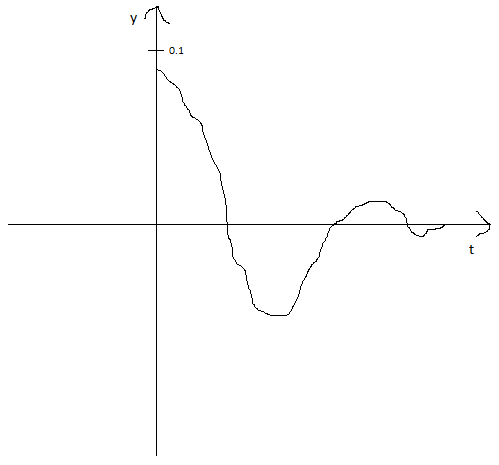
\includegraphics[width=12.6cm, height=9cm]{E17Figur_01.png}










			\subparagraph{b)}
				\begin{gather*}
v = f \lambda = 0.74 \text{Hz} \cdot 1.5 \text{m} = 1.11 \text{m$/$s}
				\end{gather*}









			\subparagraph{c)}
				\begin{flushleft}
Bruker likning Når bølgen beveger seg mot grunna vil fortsatt vanntettheten og bølgevektoren være like som tidligere. Det samme er også $g$, overflatespenningen $T$ og fjærkonstanten $k$. Det eneste som endrer seg er dybden $h$, og denne blir mindre, som fører til at bølgen brer seg saktere.
				\end{flushleft}









			\subparagraph{d)}
				\begin{flushleft}
Siden utbredelseshastigheten blir mindre og den er gitt av $v = f \lambda$ må enten både frekvensen og bølgelengden eller en av dem bli mindre. Siden vinkelhastigheten er den sammen som tidligere vil frekvensen være den samme. Det betyr at bølgelengden må bli mindre.
				\end{flushleft}









			\subparagraph{e)}
				\begin{flushleft}
Når bølgene beveger seg mot kysten kommer de inn på grunnere vann. Da senkes farten deres og de blir brutt mot kysten slik at de kommmer parallelt inn. Dette er det samme som skjer med lys når det går fra luft til vann eller luft til glass.
				\end{flushleft}








		\paragraph{3.}
			\subparagraph{a)}
				\begin{flushleft}
Et fjernt motiv blir fokusert i brennvidden, det vil si $400 \text{mm}$ unna. For å finne avstanden hvis objektet er $4.2 \text{m}$ unna bruker vi linseformelen som sier at gir at
$$\frac{1}{s} + \frac{1}{s'} = \frac{1}{f}$$
$$s = \frac{1}{\frac{1}{f} - \frac{1}{s'}} = \frac{1}{\frac{1}{400 \text{mm}} - \frac{1}{4.2 \text{m}}} = 442 \text{mm}$$
Gjør til slutt det samme for blomsten
$$s = \frac{1}{\frac{1}{f} - \frac{1}{s'}} = \frac{1}{\frac{1}{400 \text{mm}} - \frac{1}{0.6 \text{m}}} = 1200 \text{mm}$$
Dette måtte i så fall blitt ett veldig langt kamera, og veldig vanskelig å holde.
				\end{flushleft}









			\subparagraph{b)}
				\begin{flushleft}
For et objekt $5$ meter unna vil
$$s = \frac{1}{\frac{1}{f} - \frac{1}{s'}} = \frac{1}{\frac{1}{400 \text{mm}} - \frac{1}{5 \text{m}}} = 435 \text{mm}$$
Forskjellen mellom denne verdien og den for uendelig langt unna er $35 \text{mm}$. Det vil si at kikkerten må kunne justeres $3.5 \text{cm}$. Den eneste forskjellen på kikkert med konveks og konkav linse er at okularet har motsatt fortegn på brennvidden. Det vil si at du fortsatt må kunne endre lengden med $3.5 \text{cm}$
				\end{flushleft}









			\subparagraph{c)}
				\begin{flushleft}
Forstørrelsen $M$ er gitt ved $M = - \frac{f_1}{f_2} = \frac{400 \text{mm}}{50 \text{mm}} = - 8$. For konkave linse blir fortegnet motsatt.
				\end{flushleft}









			\subparagraph{d)}
				\begin{flushleft}
Konkav linse gjør at bildet blir riktig vei og at kikkerten blir kortere.
				\end{flushleft}









			\subparagraph{e)}
				\begin{flushleft}
Rayleighs oppløsningskriterium sier at
$$\Psi = \frac{1.22 \lambda}{D} = \frac{1.22 \cdot 500 \text{nm}}{50 \text{mm}} = 1.22 \cdot 10^{-5}$$
Dette tilsvarer
$$1.22 \cdot 10^{-5} \cdot \frac{180}{\pi} = 0.000699^{\circ} = 2.5164''$$ \\
Dette er akkurat på grensa, så jeg tipper vi vil bare se to, men kan hende tre hvis du har veldig gode øyne.
				\end{flushleft}









			\subparagraph{f)}
				\begin{flushleft}
Fargene blir skarpe ved forskjellige avstander, så noe av blomsten vil være skarp der andre ikke vil være det. Dette kalles kromatisk aberrasjon.
				\end{flushleft}









			\subparagraph{g)}
				\begin{flushleft}
Fordi dette er kantene på linsa til kikkerten, som gir en annen utforming på linsa.
				\end{flushleft}








		\paragraph{4.}
			\subparagraph{a)}
				\begin{flushleft}
Løst på papir, bruker Faradays lov, tar $\nabla X$ på begge sider og benytter sammenhengen i oppgaven. Bytter om på derivasjonsrekkefølgen og gjør bruker deretter Amperé/Maxwells lov ved innsetting av $B = \mu_r \mu_0 H$ og $E = \epsilon_r \epsilon_0$. Til slutt antar jeg at det ikke er noen fri ladning eller stømning. Da stemmer alt
				\end{flushleft}









			\subparagraph{b)}
				\begin{flushleft}
Også gjort på papir, men enkel hvis du bruker løsningen av bølgelengden
$$E = E_0 e^{i (kx - \omega t)}$$
og at $v_f = \frac{\omega}{k}$ i tilleg til likningener som står på formelarket og løsningen for bølgelikningen ved tid $t = 0$ og $x = 0$.
				\end{flushleft}









			\subparagraph{c)}
				\begin{flushleft}
$k = \frac{2 \pi}{\lambda} = \frac{2 \pi}{30 \text{m}} = 0.21 \text{m}^{-1}$. Dette gir oss $\omega(0.21 \text{m}^{-1}$ som ikke vi kan lese av i dette diagrammet
				\end{flushleft}
\end{document}